\documentclass[12pt]{article}
\usepackage[hidelinks]{hyperref}    
\usepackage[all]{hypcap}   
\usepackage{graphicx}
\usepackage{amsmath}
\graphicspath{{../images/}}
\author{Andrea Malvezzi}
\title{\textbf{Architettura degli Elaboratori~-~Rappresentazione dell'informazione}}
\date{04 Ottobre, 2024}
\author{Andrea Malvezzi}
\begin{document}
\maketitle
\pagebreak
\tableofcontents
\pagebreak
\section{Codifiche e sistemi di numerazione}
I calcolatori elaborano tipi diversi di informazioni, ma alla base di ognuna di queste categorie ci sono i bit della memoria, ovvero dei valori binari.\\
Per convertire i dati dalla loro "forma originale" a un qualcosa di comprensibile dal calcolatore (ovvero sequenze di zero e di uno), occorre una codifica.
\subsection{Sistemi di numerazione posizionali}
Una codifica ha una \textbf{base} $b$, a cui corrisponde un quantitativo di caratteri con cui codificare i valori da convertire in un certo formato.\\
Ad esempio, la codifica binaria ha base $2$, in quanto utilizza solamente lo $0$ e l'$1$.\\
Altre codifiche importanti sono quella ottale (base 8) ed esadecimale (base 16, dal 9 in poi si usano le lettere in ordine alfabetico).
\subsection{Leggere un numero in una certa base}
Avendo un numero codificato in base $b$, allora tale numero corrisponderà a:
\begin{equation}
    \sum_{i=0}^{k} d_i \cdot b^i    \label{formula:leggere_codifica}    
\end{equation}
\subsubsection{Esempio di diversi tipi di codifica}
Prendiamo come esempio il numero 2001 in base decimale (quella con cui siamo abituati a contare nella matematica "standard").\\
Ora convertiamolo in binario, ottale e esadecimale:
\[
    2001_{10} = 11111010001_2
\]
In quanto il primo uno corrisponde a $1*2^{10}$, il secondo a $1*2^9$, e così via, fino all'ultimo che corrisponde a $1*2^0$, quindi a 1.
\[
    2001_{10} = 3721_8
\]
\[
    2001_{10} = 7D1_{16}
\]
Tutte queste 3 codifiche sono \textbf{equivalenti}, in quanto rappresentano tutte lo stesso numero.
\subsection{Metodi alternativi per effettuare conversioni}
Per convertire un numero in binario da decimale, basta dividerlo per 2 e segnare i resti:
\begin{gather*}
    2999 : 2 = 1499, \text{ con resto pari a } 1.\\
    1499 : 2 = 749, \text{ con resto pari a } 1.\\
    \text{etc} \dots \\
    5 : 2 = 2, \text{ con resto pari a } 1\\
    2 : 2 = 1, \text{ con resto pari a } 0
\end{gather*}
Mentre per fare la conversione inversa, si può optare per un metodo più alternativo, ovvero quello delle \textbf{moltiplicazioni successive}:
\begin{figure}[!htb]
    \centering
    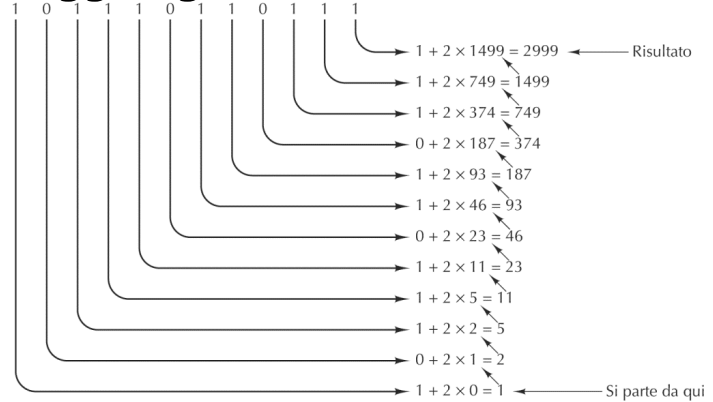
\includegraphics[width=.9\linewidth,height=.40\textheight,keepaspectratio]{rappresentazione_dati/mult_succ.PNG} % essenzialmente resiza l'immagine
    \begin{center}
        \caption{\label{fig:moltiplicazioni_successive}Partendo da sx e con un moltiplicatore pari a 0, per ogni cifra si somma la cifra in questione al doppio del moltiplicatore, per poi assegnare al moltiplicatore valore pari a quello appena ottenuto.}
    \end{center}
\end{figure}
\end{document}